% Chapter Template

\chapter{Software Implementation} % Main chapter title

\label{c:soft-impl} % Change X to a consecutive number; for referencing this chapter elsewhere, use \ref{ChapterX}

%----------------------------------------------------------------------------------------
%	SECTION 1
%----------------------------------------------------------------------------------------

\section{Overview}
 

 
\begin{lstlisting}
some code
//goes here
\end{lstlisting}

\addfigure{0.8}{ovFull.pdf}{Sequence diagram depicting\ldots}{f:ovFull}

\subsection{Monitor tasks}
The monitor tasks must run on the FTC. They consist of:
\begin{itemize}
  \item setting up task parameters and initializing all critical task models
  \item managing dataflow between tasks 
  \item intercore task communication 
  \item retrieving valid data when critical tasks execute correctly on other resources 
  \item restarting cores in the case of a transient fault
  \item managing the global data space
  \item organizing coordinated virtual memory management and memory protection between cores to achieve correct fingerprinting
\end{itemize} 

Figure~\ref{f:monitor-send} shows a high-level view of how the interaction between monitor tasks in order to send a message.

\begin{figure}
\centering
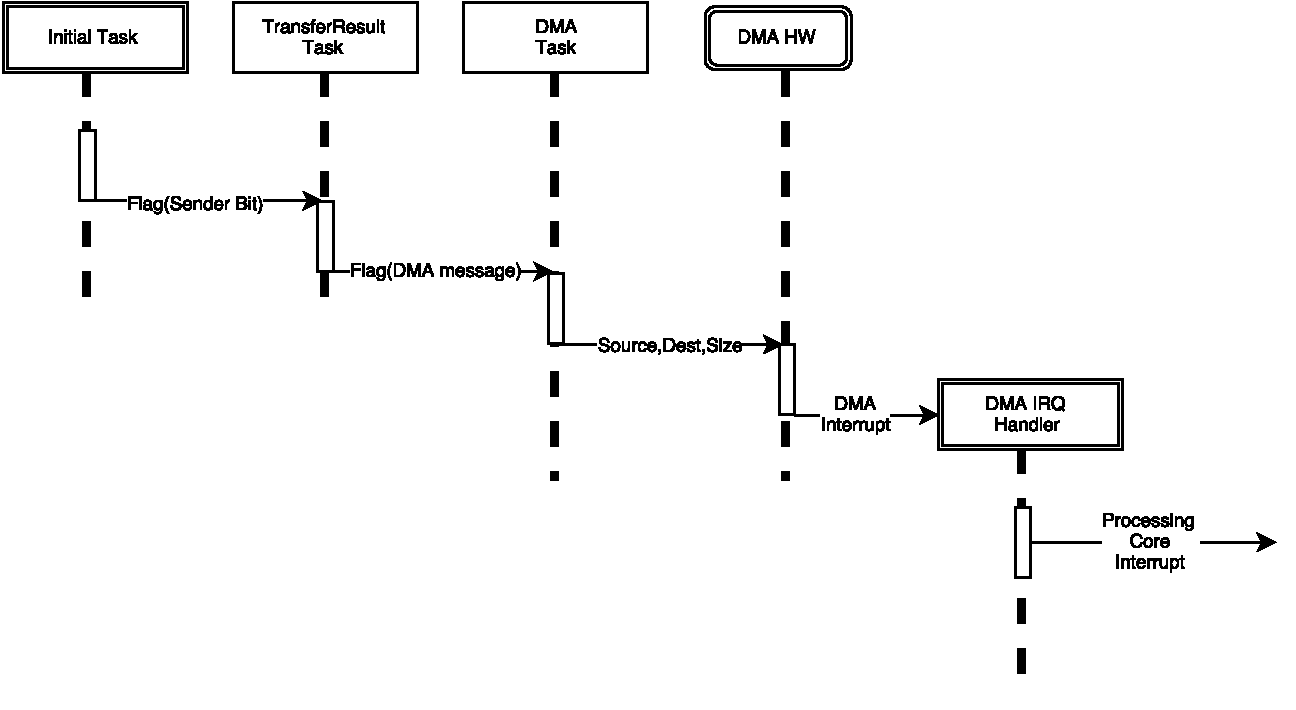
\includegraphics[scale=0.7]{monitor-send.pdf}
\caption{The interaction between monitor tasks when setting up a critical task to run on another core}
\label{f:monitor-send}
\end{figure}
